\chapter{Implementation and Design}
The uneven illumination, particularly high dynamic lighting environment, causes many problems.
For example, the images acquired by digital cameras, camcorders, or other terminals tend to be too
bright or dark in certain areas, the target is difficult to be identified and some other issues. 

To solve the problems for the quality of image acquisition caused by uneven illumination, a
series of methods had been put forward successively, including histogram equalization, image
enhancement in gradient field, homomorphic filter and the Retinex theory. Among these methods,
the Retinex has become a research hotspot recently as it could achieve a good balance in dynamic
range compression, edge enhancement and color constancy. There are three classical algorithms
based on the Retinex theory\cite{retinex}, they are SSR (Single Scale Retinex), MSR (Single Scale Retinex) and MSRCR (Multi-Scale Retinex with Color Restoration)\cite{retinex}. However, SSR could only choose one dimension, it was difficult to simultaneously ensure the dynamic range compression and color
fidelity\cite{retinex}. Although MSR can ensure the dynamic range compression and color fidelity, it could not achieve the high color fidelity, as it simply weighted the different scales linearly. While MSRCR could achieve color fidelity much further, it was not conducive to real-time applications,
because a lot of parameters needed to be set. Furthermore, the above three algorithms may
produce halo and color distortion in high contrast regions, since the illuminant image was
obtained by Gaussian low-filter. 
In order to overcome such problems as halo and color distortion for the traditional Retinex, many
improved algorithms have been proposed. For example, the halo was reduced through bilateral filter
to obtain the illuminant image, but due to being ignorant of the correlations between each channel
of the color image, it could not decrease the color distortion. However, it was not conducive to real-time application, as a lot of parameters needed to be set\cite{msr1}.

\section{Retinex theory and its typical algorithms }
Retinex (abbreviation of Retina and Cortex) theory is a model been used to explain how the
human visual system perceive color and brightness of objects. It is also the interpretation of
color constancy indicating the color of the same objects is constant, though they are under different
lighting. Briefly, the basic principle of Retinex theory \cite{retinex} is that the original image can be divided into illuminant and reflected image, and the enhancement can be achieved through reducing the effects of illuminant image on the reflected. As shown as in formula \eqref{fig:illumination} 

\begin{equation}
	S(x,y)=R(x,y)*L(x,y)
	\label{fig:illumination}
\end{equation}

Where $L(x,y)$ represents incident light or illuminant image deciding the dynamic range
achieved by image pixels $R(x,y)$ represents reflective properties or reflected light deciding the
interior properties of image $S(x,y)$ represents the original image. And the visual effects can be
improved, mainly by obtaining the reflective properties or reflected image \cite{retinex}. 

\subsection{Single Scale Retinex(SSR)}
The SSR algorithm based on center/surround Retinex approved by Edwin Land is firstly
improved and realized by Jobson and his colleagues\cite{retinex}. And the illuminant image is also obtained by Gaussian low filter as in formula \eqref{fig:ssr}\cite{ssr}.
\begin{equation}
	R_{SSR}(x,y)=\log S(x,y) - \log (S(x,y) \otimes F(x,y))
	\label{fig:ssr}
\end{equation}

Where the symbol $\otimes$ represents convolution operation. $F(x, y)$ is Gaussian surrounding
function in the following formula\cite{retinex}
\begin{equation}
	F(x,y)= \gamma \; exp(- \frac{(x^{2}+y^{2})}{\sigma^{2}}
	\label{fig:ssr1}
\end{equation}

\begin{equation}
	\iint F(x,y)dxdy = 1
	\label{fig:ssr2}
\end{equation}


Where $\gamma$ is a normalization constant, $\sigma$ is the scale of surrounding function, and the smaller $\sigma$ is, the more contrast is enhanced, but the more distinct the halo phenomenon becomes.
Conversely, the larger $\sigma$ is, although the less contrast is enhanced, the more effectively the halo is suppressed. Large numbers of experiments indicate that, if $\sigma$ is between 80 and 100, the balance can be maintained\cite{retinex}.
\clearpage
\section{Design}
\subsection{Flow Chart}

\begin{figure}[!htb]
	\centering
	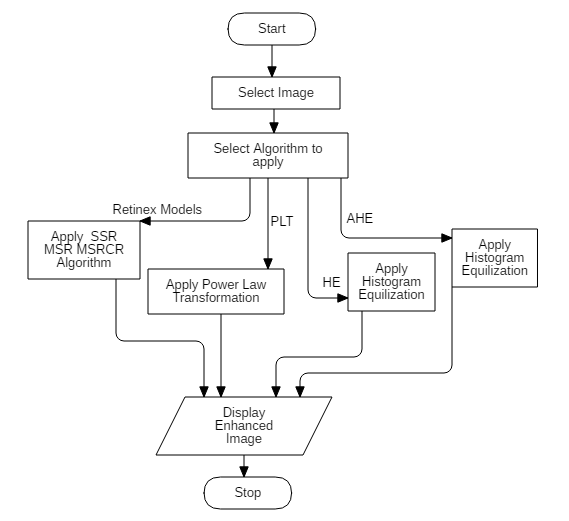
\includegraphics[scale=0.6]{images/ch4/flowChart.png}
	\caption{Flow chart for Image Enhancement}
	\label{fig:flowChart}
\end{figure}


\subsection{Activity Diagram}

\begin{figure}[!htb]
	\centering
	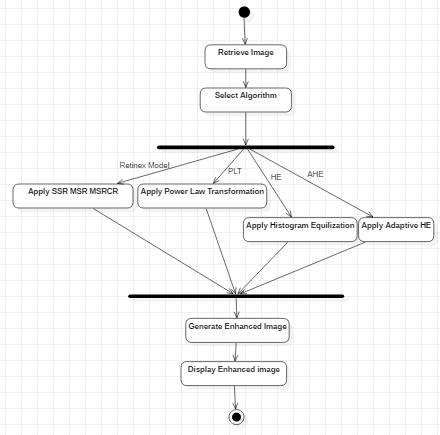
\includegraphics[scale=0.7]{images/ch4/activity.png}
	\caption{Activity Diagram for Image Enhancement}
	\label{fig:activity}
\end{figure}


\subsection{Deployment Diagram}

\begin{figure}[!htb]
	\centering
	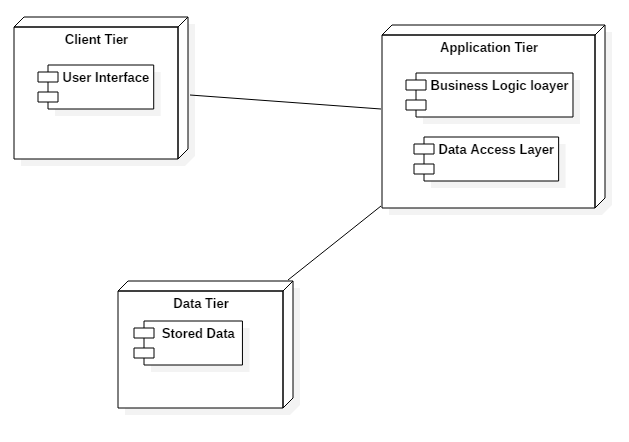
\includegraphics[scale=0.8]{images/ch4/deployment.png}
	\caption{Deployment Diagram for Image Enhancement}
	\label{fig:deployment}
\end{figure}


\subsection{Component Diagram}

\begin{figure}[!htb]
	\centering
	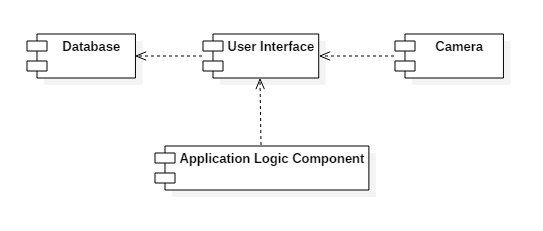
\includegraphics[scale=0.8]{images/ch4/component.png}
	\caption{Component Diagram for Image Enhancement}
	\label{fig:component}
\end{figure}
